\documentclass[12pt,a4paper]{article}
\usepackage[utf8]{inputenc}
\usepackage{geometry}
\usepackage{titlesec} % For customizing section titles
\usepackage{graphicx} % For images
\usepackage{hyperref} % For hyperlinks
\usepackage{fancyhdr} % For fancy headers and footers
\usepackage{lipsum} % For generating dummy text

% Set page geometry
\geometry{left=2.5cm, right=2.5cm, top=2.5cm, bottom=2.5cm}

% Set up hyperref
\hypersetup{
    colorlinks=true,
    linkcolor=black,
    filecolor=magenta,
    urlcolor=cyan,
}

% Customize section titles
\titleformat{\section}{\large\bfseries}{\thesection}{1em}{}
\titleformat{\subsection}{\normalsize\bfseries}{\thesubsection}{1em}{}

% Setup headers and footers
\pagestyle{fancy}
\fancyhf{}
\rhead{3D printing defect detection}
\lhead{AI Project Proposal}
\rfoot{Page \thepage}

% Title and author
\title{\textbf{ AI Project Proposal 3D printing defect (spaghetti) detection}}
\author{Michal Raczkowski}
\date{10-01-2024}

\begin{document}

\maketitle
\thispagestyle{empty} % Remove header/footer for the first page

% Insert table of contents
\newpage
\tableofcontents
\newpage

\setcounter{page}{1} % Start page numbering from here

\section{Introduction}
Since 3D printing appeared for personal consumers, one of the main problems with this technology was its tendency to fail, especially with inexperienced users and early versions of 3D printers. Although through the years the technology has improved significantly, it is still unpredictable and requires assistance due to material waste and safety concerns.

\section{Domain Understanding}
\subsection{Objective}
Goal of the project is to detect certain kind of defect in 3D print (FFF) model based on image recognition
\subsection{Background}
Fused Filament Fabrication (FFF) is a popular 3D printing method where a thermoplastic filament is heated to its melting point and then extruded, layer by layer, to build a three-dimensional object. This process begins with a digital 3D model, which is sliced into thin layers by specialized software. The 3D printer then precisely deposits the melted filament according to these layers, typically using a moving print head. As each layer solidifies, the print bed or the print head moves to allow the next layer to be added directly on top. FFF is favored for its versatility in using a wide range of materials, ease of use, and affordability, making it ideal for both hobbyists and professionals for creating prototypes, functional parts, and artistic objects.
\subsection{Exploratory Research}
The problem with Fused Filament Fabrication (FFF) 3D printing technology is that the machine sometimes malfunctions, causing the deposition of plastic in incorrect places, which leads to various defects. Additionally, if the model is not properly adjusted for 3D printing, it can also cause defects. These various types of defects can lead to excessive material waste or safety concerns.

\section{Data Sourcing}
\subsection{Data Relevance}
Relevant data to achieve the objective of this project would include a series of images displaying certain defects on various types of 3D printed models.
\subsection{Data Characteristics}
% Describe the types and volume of data you need.
All data would be pictures in preferred formats like \verb|.jpeg| or \verb|.png|, and in proffered size 
\subsection{Data Collection Methods}
Data would be collected from homemade pictures displaying failing prints with certain defect and from online open sources 
\subsection{Challenges \& Solutions}

% Introduction to the challenges
The challenges faced in this area include

\subsubsection{Homemade pictures}
\begin{itemize}
    \item Challenges
    \begin{enumerate}
        \item Time consuming process of creating prints with defects
        \item Interfering lighting 
        \item Interfering background
    \end{enumerate}
    \item Solutions
    \begin{enumerate}
        \item Use smaller models, and decreased quality of prints to speed up process of printing
        \item Use of artificial source of light
        \item Use of constant homemade background e.g. cardboard
    \end{enumerate}
\end{itemize}

\subsubsection{Online sourced pictures}
\begin{itemize}
    \item Challenges
    \begin{enumerate}
        \item Copyright laws
        \item Display different types of defects then preferred one
        \item Low quality pictures
        \item Wrong format of pictures 
    \end{enumerate}
    \item Solutions
    \begin{enumerate}
        \item Use pictures which are free to use, or are on creative commons and public domain laws 
        \item Choose pictures which displays proffered defect  
        \item Chose pictures which fits minimal requirement of resolution and do not contain interfering lighting or background
        \item Choose pictures in preferred format like \verb|.jpeg| or \verb|.png| 
    \end{enumerate}
\end{itemize}


\section{Analytic Approach}
\subsection{Target Variable}
Goal of this project is to detect specific defect where a print fails, resulting in a mess of extruded filament that resembles spaghetti, as shown in Figure~\ref{fig:spaghetti3D} This occurs when the print doesn't adhere properly to the build plate or when a part of the print moves or detaches during the printing process. As the printer continues to extrude filament, it deposits the material in a disorganized manner, creating a tangle of filament.

\begin{figure}[h]
    \centering
    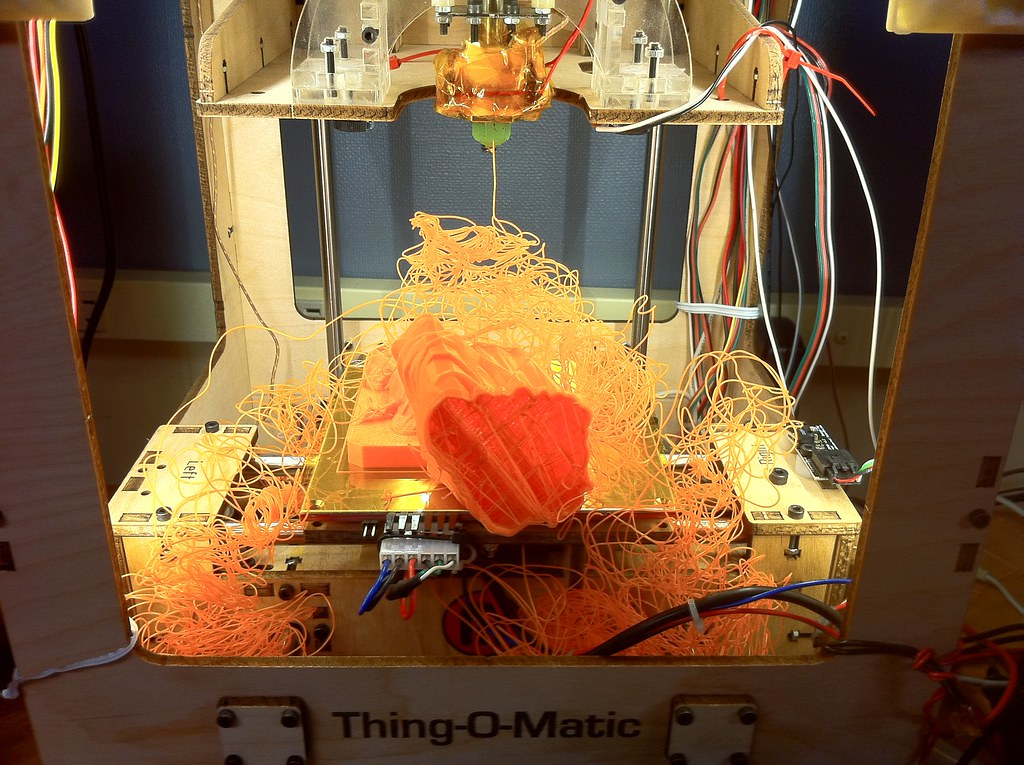
\includegraphics[width=0.8\linewidth]{spaghetti3D.jpg}
    \caption{Extruded filament that resembles spaghetti}
    \label{fig:spaghetti3D}
    \end{figure}

\subsection{Problem Nature}
Nature of this problem is classification because we have to classify if spaghetti defect appeared on picture
\subsection{Indicators}
The picture shows an unordered structure of plastic filament, which resembles spaghetti, instead of a correctly structured model.

\section{Data Preparation}
\subsection{Preprocessing Needs}
To create proper dataset we need to 
\begin{itemize}
    \item Standardize size of images
    \item Standardize format of images
    \item Normalize pixels values (usually to the range [0, 1] or [-1, 1]) to facilitate neural network training.
    \item Create annotations
    \item Create label files with annotations
\end{itemize}
\subsection{Tools \& Techniques}
\begin{itemize}
    \item Cropping images
    \item Converting images to chosen format
    \item Python
    \item Use annotation tools such as LabelImg or VOTT for annotation
\end{itemize}

\section{Modeling}
\subsection{Proposed Models}
The main model planned for use is YOLO (You Only Look Once), and the aim is to explore its different variants such as YOLOv3, YOLOv4, etc.
\subsection{Evaluation Metrics}
% Define how you'll measure the model's performance.
\begin{itemize}
    \item \textbf{Intersection over Union (IoU):}  IoU is a measure that quantifies the overlap between a predicted bounding box and a ground truth bounding box. It plays a fundamental role in evaluating the accuracy of object localization.
    \item \textbf{Average Precision (AP):} AP computes the area under the precision-recall curve, providing a single value that encapsulates the model's precision and recall performance.
    \item \textbf{Mean Average Precision (mAP):} mAP extends the concept of AP by calculating the average AP values across multiple object classes. This is useful in multi-class object detection scenarios to provide a comprehensive evaluation of the model's performance.
    \item \textbf{Precision and Recall:} Precision quantifies the proportion of true positives among all positive predictions, assessing the model's capability to avoid false positives. On the other hand, Recall calculates the proportion of true positives among all actual positives, measuring the model's ability to detect all instances of a class.
    \item \textbf{F1 Score:} The F1 Score is the harmonic mean of precision and recall, providing a balanced assessment of a model's performance while considering both false positives and false negatives.
\end{itemize}

\section{Conclusion}

Final result of this project can help to prevent creating defected models and waste of material. It also can increase safety of whole process of 3D printing 

\end{document}
